\section{Introduction}
\label{sec:introduction}
Machine Learning (ML) is the area of artificial intelligence (AI) which involves the development of models that are trained on data to perform specific tasks. The last years have shown great improvements in model's capabilities in extracting useful information from images. Societal regulations for the technology and consumer opinions with regards to privacy and data security is struggling to keep up with the rapid increase in complexity and capabilities of the developed and deployed machine learning models. 

On-device processing is emerging as a vital component of modern human detection and tracking systems, particularly as a strategy to enhance privacy and data security. The ability to detect and track humans in real-time is essential across a range of applications, from security surveillance to visitor analytics in cultural institutions. However, the deployment of these systems, especially in sensitive environments like museums and aquariums, raises significant privacy and data security concerns. This thesis explores the development and deployment of a privacy-preserving human localization system, specifically addressing the challenges posed by on-device processing where images are deleted or obfuscated post-inference. This process complicates the validation of inference accuracy, especially since many models trained on large, generic datasets may not perform equivalently in specific deployment scenarios. A dataset was collected, and analysis on live data was performed (see Figure \ref{fig:example_from_aquarium}).

\begin{figure}[H]
    \centering
    \begin{subfigure}{0.475\textwidth}
        \centering
		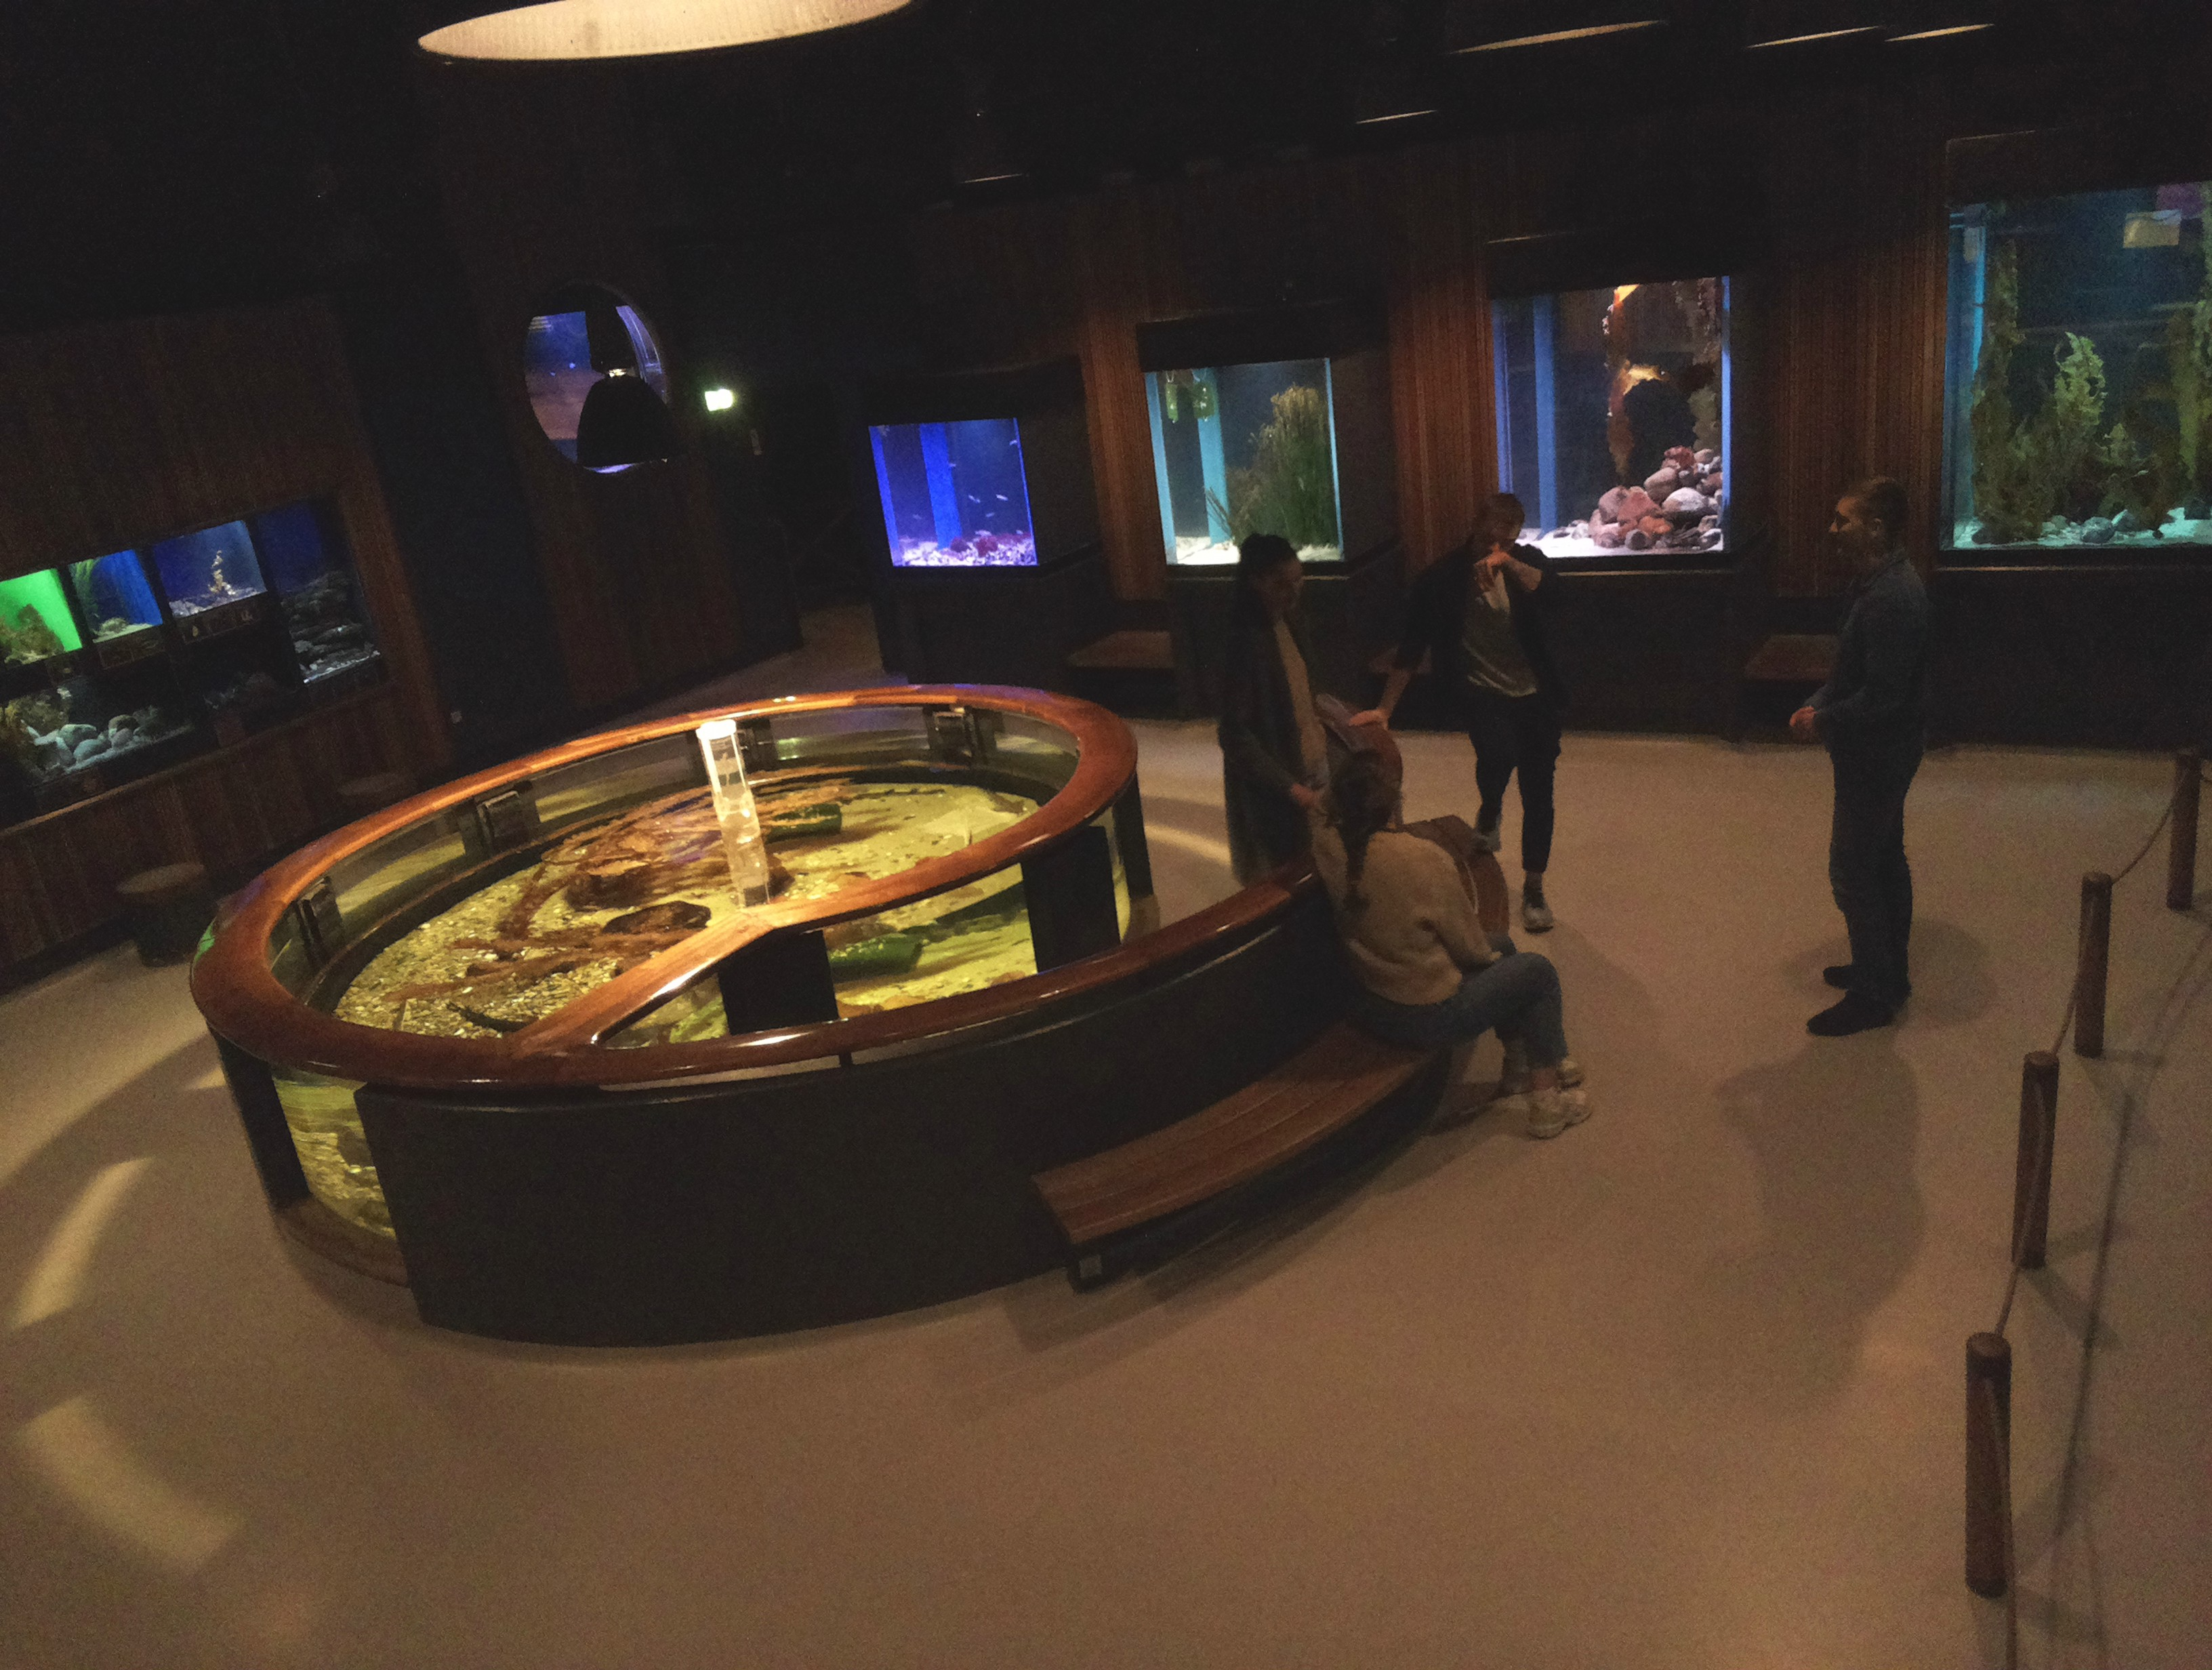
\includegraphics[width=\textwidth]{Images/DeviceImages/2nd-iteration/example.jpg}
        \caption{Example Image From the FIMUS Dataset.}
    \end{subfigure}
    \hfill
    \begin{subfigure}{0.475\textwidth}
        \centering
        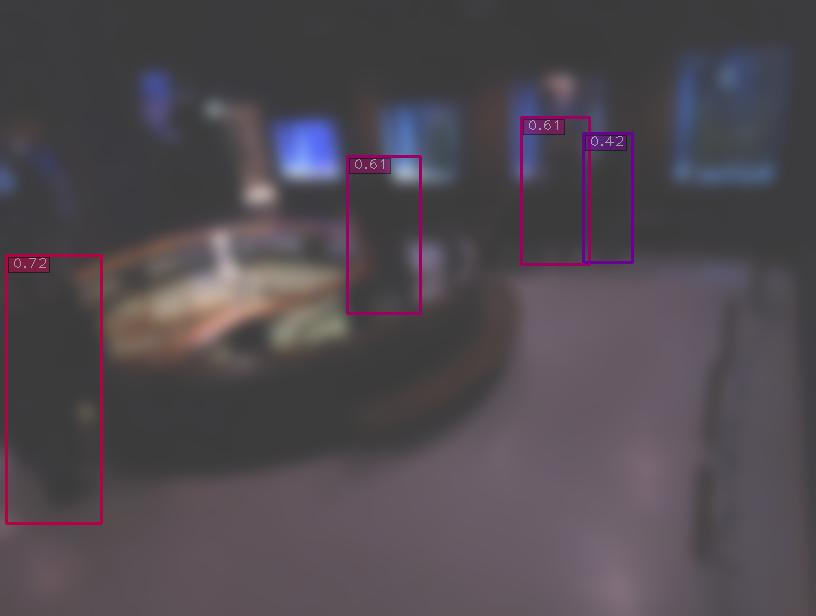
\includegraphics[width=\textwidth]{Images/DeviceImages/live-example.jpg}
        \caption{Example Image From the Live Detections.}
    \end{subfigure}
	\caption{Example Images From the FIMUS Aquarium. }
	\label{fig:example_from_aquarium}
\end{figure}
todo bytt ut med et b med de rette innstillingene?

% \subsection{Background and Motivation}
\subsection{Problem Description}
The method of human detection and tracking in public spaces has significantly evolved over the past decade, driven by advancements in computer vision and machine learning. Traditional surveillance systems typically relied on centralized processing, where video feeds were transmitted to a remote server for analysis. This approach not only raised privacy concerns due to the potential exposure of sensitive information but also required substantial human intervention, making it time-consuming, error-prone, and lacking in scalability. This thesis advocates for a shift towards \textit{on-device} processing, which performs analytics locally on the edge device, thereby eliminating the need to transmit raw video data and significantly enhancing privacy. This is particularly relevant for environments such as museums and aquariums where privacy preservation is critical.

Additionally, the performance of object detection models is often evaluated using generic datasets like COCO, which may not accurately reflect the conditions of the deployment environment. This discrepancy can lead to suboptimal model performance in real-world scenarios, where factors like lighting conditions, camera angles, and object occlusion can significantly impact detection accuracy. This thesis aims to investigate the impact of using deployment-specific data for the fine-tuning of object detection models, and on the evaluation of object detection models, comparing the performance metrics obtained with those from generic datasets.

\subsection{Scope}
To demonstrate the feasibility and effectiveness of on-device human detection and localization in a practical setting, two devices were deployed in the "Fiskeri og Søfartsmuseet" (FIMUS) aquarium in Esbjerg, Denmark. The deployment aimed to address the unique challenges of indoor, low-light environments. A dataset of 3397 images was collected and labeled, and was used to evaluate and fine-tune several object detector machine learning models. An example image from the aquarium is displayed in Figure \ref{fig:example_from_aquarium}. The best performing model was subsequently deployed to collect anonymous data on visitors over a month, with results visualized through heatmaps and analysis of peak visitation hours. 

The scope of this project is dualistic. It encompasses demonstrating a comprehensive implementation of a privacy-preserving human localization system. It also encompasses critically assessing the validity of object detection model performances across general and specific datasets to understand the real-world impacts of scientific advancements. 

The focus of this thesis is selectively deep on topics such as privacy, privacy preservation in images, and performance metrics of object detectors. These areas are emphasized due to their critical relevance and the necessity of a fundamental understanding of these topics to grasp the project's core objectives. While other subjects like object detector model architecture, edge devices, challenges in object detection, security, and decision support systems also present interesting avenues of exploration, they are not central to the thesis' primary aims.

This thesis is intended for a diverse readership, including edge-device engineers, AI and machine learning enthusiasts, non-technical social studies scholars, and policymakers engaged in crafting regulations for object detection technologies. This results in a broad scope of topics covered in the thesis, ranging from technical discussions on machine learning models to ethical considerations in deploying object detection systems in public spaces.

The project of this thesis also spanned several disciplines. It required research, development, and effort in edge-device deployment, machine learning, and data science. Choices were made to focus the scope to manage the workload effectively.

\subsection{Limitations}
\paragraph{Secure Control of Device}
\phantomsection
\label{sec:scope_ssh}
A dataset was built of consenting individuals in an aquarium which was part of a larger museum facility. However, once development was finished and the system was tested, the devices were actively photographing individuals who had \textit{not} given consent to be photographed. Privacy was still preserved by immediately inferencing on and deleting the images. In such an application, it is imperative to not store or upload clear, privacy-intrusive images. Therefore, an existing and already proven secure solution developed by \textit{HallMonitor}, a company specializing in on-device processing solutions based in Esbjerg, was utilized to establish a secure communication channel with the deployed devices. The communication channel was used to extract the analytics data from the devices. This secure system setup, necessary to protect the devices from attackers, is not covered in this thesis due to its proprietary nature.

\paragraph{Legal Considerations}
The discussions and insights in this thesis may apply to global applications, but the legal considerations specifically target the European Union member countries. Further, some of the discussions may be influenced and biased by a heavily european-influenced cultural mindset and thus not be as relevant and applicable to parts outside Europe. More detailed discussions on international privacy laws beyond just the GDPR should have been included if the technology was intended for global application.

\paragraph{Fine-tuned Model Development}
The project's broad scope resulted in a limited exploration of potential improvements in model fine-tuning. This thesis evaluates the performance of various machine learning models, including models built from the three arhitectures YOLOv3, YOLOv9, and DETR. Two more object detection architectures are also mentioned, but were not (fully) implemented. These are Co-DETR, the current best-performing model on the COCO dataset, and the Faster-RCNN, another popular and good option for object detection. However, the Co-DETR was deemed too complex and resource-intensive for the project's scope to be fully implemented and evaluated, and Faster-RCNN was not prioritized due worse performance than the YOLOv9. The object detectors are discussed in Section \ref{sec:object_detection}.

\paragraph{Museum and Aquarium Opening Hours and Visitor Conduct}
\phantomsection
\label{sec:scope_opening_hours}
The project was designed to avoid interference with the normal operations of the aquarium. Consequently, image capture for the dataset was confined to aquarium opening hours, and random visitors were not inquired whether they'd be willing to participate in the project. An early analysis of the visitation patterns revealed the aquarium was busy from the opening at 10:00 until approximately to 15:00, 2 hours before closing time. This meant most images for the dataset were captured in the two hours before closing time where there was least traffic.

\paragraph{The Task is Object Detection}
\phantomsection
\label{sec:scope_object_detection}
There are several tasks within the domain of computer vision, each serving distinct purposes and complexities. This project focuses exclusively on simple object detection, which involves locating objects of relevance within an image. Specifically, this thesis addresses single-class object detection with \textit{person} as the sole class of interest. Other tasks in computer vision include person re-identification, image classification, combined image classification and localization, semantic segmentation, and instance segmentation. Re-identification involves recognizing individuals across different images and image classification is the task of classifying the image contents as a whole. The rest of the tasks are illustrated in Figure \ref{fig:computer_vision_tasks} to display how they differentiate from object detection. 

\begin{figure}[H]
    \centering
    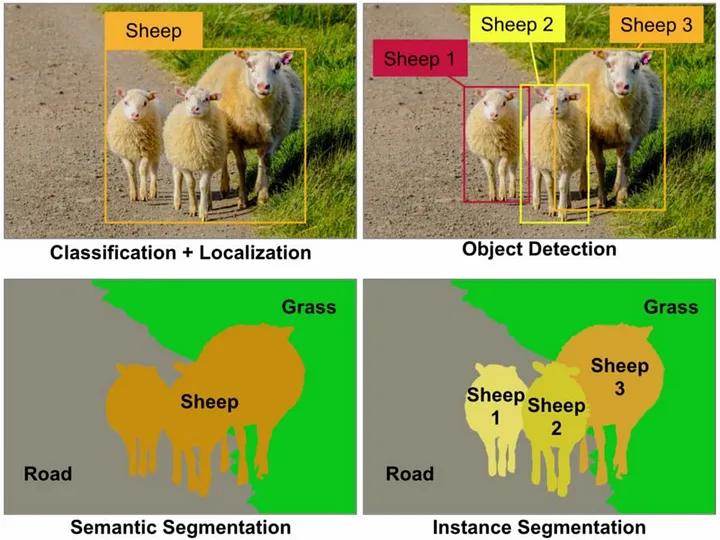
\includegraphics[width=0.6\linewidth]{Images/computer_vision_tasks.png}
    \caption{Image processing tasks (\cite{mu2021object_detection_operations}).}
    \label{fig:computer_vision_tasks}
\end{figure}

The selection of a dataset must be directly aligned with the specific task to be performed, as it must contain data suited for that task. For instance, applications tasked with person reidentification require a dataset that includes the identities across images for the persons depicted in the images. An appropriate dataset for such applications, the Person Reidentification in the Wild (PRW), is detailed in Section \ref{sec:dataset_PRW}.

\paragraph{Lighting Conditions in Aquarium Settings}
\phantomsection
\label{sec:scope_aquarium_light}
The environmental conditions within aquarium settings impose specific lighting requirements that significantly influence the deployment and performance of the proposed object detection system. Aquariums typically maintain low-light conditions, presumably to minimize stress for the aquatic animals and improve vision into the tanks for the visitors. In this context, the options for enhancing illumination are often limited, making it impractical to simply increase lighting to facilitate better visual detection technologies. These subdued lighting conditions were an important feature of the thesis project.

\paragraph{TinyML and Frugal Devices}
\phantomsection
\label{sec:scope_tinyML}
An initial attempt was made to encompass tinyML and frugal devices in the project. TinyML is when machine learning models are aimed at deployment to heavily resource-constrained environments, e.g. "frugal devices". These are devices where the microcontroller units (MCUs) are accompanied by memory measured in kilobytes, and processor speeds measured in megahertz. Machine learning networks applied to tiny robots are subject to challenges from size, weight, area, and power (SWAP) (\cite{ne2022robotstinymlconstraints}). Many of the same challenges apply even in applications where the SWAP challenges are not the main concerns. \citeauthor{ra2023reformabletinyml} mentions the open challenges and future directions of the next generation tinyML. Catastrophic forgetting, which is when information from previous tasks while learning new ones are forgotten, are a result of the frugal devices' computational resources and memory\footnote{Catastrophic forgetting can also be seen in transfer learning, and is why freezing the backbone of a pre-trained model may be a good idea.}. The first recommendation for future directions from the authors is to investigate fog computing as a means to offload tasks from the frugal devices. Exploring a system of frugal devices for obtaining sensor data on the edge and "fog devices"\footnote{Fog devices is an unofficial term for processing-instances located close to the edge.} for processing of the data would be a time-consuming objective, especially in a real-world scenario where security must be taken seriously. Therefore, tinyML and frugal devices are not elaborated in detail in this thesis, but discussed briefly in \ref{app:tinyML}. 

\paragraph{Model Hyperparameter Tuning}
\phantomsection
\label{sec:scope_hyperparameter_tuning}
The project did not encompass hyperparameter tuning of the models. Hyperparameter tuning is the process of finding the best hyperparameters for a machine learning model. Hyperparameters are the settings of the model that are not learned from the data, such as the learning rate, batch size, and number of epochs. Hyperparameter tuning is a crucial step in the machine learning pipeline, as it can significantly impact the model's performance. However, due to time and resource constraints, hyperparameter tuning was not included in this project. Further comments on hyperparameter tuning are made in Section \ref{sec:hyperparameter_tuning}.

\subsection{Research Questions}
\label{sec:research_questions}
Rather than forming a single hypothesis for this rather widespread project, a set of research questions are formulated to guide the research and to provide a structured approach to the investigation.

% The hypothesis of the thesis is that the dataset quality will have an impact on fine-tuned model accuracy, and that the deployment-specific test data will rank the models similarily to the ranking we see on the general datasets. todo hypothesis her bladnes entall og flertall... bestemt/ubestemt..Kanskje del av secondary objectives?

\textbf{The Research Questions are as follows:}
\begin{enumerate}
	\item What are some privacy risks associated with traditional human localization systems in public spaces, and how may a system mitigate these privacy concerns?
	\item How does the validity of object detection model evaluations change when using data specifically from the intended deployment environment compared to using generic datasets?
	\item What are some machine learning architectures suitable for object detection in a real-world deployment scenario?
	\item How many images are needed for testing before the average precision of a machine learning model converges in a single-environment setting?
\end{enumerate}

\subsection{Research Objectives}
\label{sec:research_objectives}
\textbf{The Primary Objectives are to:}
\begin{enumerate}
	\item Develop a privacy-preserving human localization system using on-device processing to minimize data transmission and enhance data privacy.
	\item Demonstrate feasability and effectiveness of on-device human detection and tracking in a practical and realistic setting.
	\item Investigate the effects of the dataset quality in fine-tuning of models on the performance.
	\item Assess the impact of using real world-specific test data on the evaluations of object detection models, by comparing model evaluations obtained with specific test data to evaluations obtained with more general datasets.
\end{enumerate}

\textbf{The Secondary Objectives are to:}
\begin{enumerate}
	\item Compare the privacy and performance impacts of on-device processing against traditional centralized processing methods.
	\item Investigate the feasibility of deploying the developed system in other public spaces to enhance visitor analytics.
	\item Demonstate how to visualize object detection data by creating visualizations of collected data from a realistic setting.
	\item Explore relevant object detection architectures to evaluate their performance in a real-world deployment sceneario.
\end{enumerate}

\subsection{Project Work}
\label{sec:action_points}
\textbf{In order to achieve these objectives, the following project work was executed and is detailed in this thesis:}
\begin{itemize}
    \item Designed and implemented a prototype system that incorporates on-device processing for privacy-preserving human localization.
    \item Deployed a prototype in an aquarium to gather real-world data and analyze system performance.
    \item Collected and labeled a dataset of 3394 images to evaluate and fine-tune several object detector machine learning models.
    \item Conducted comparative studies to evaluate the effects of data specificity and quality on model accuracy.
    \item Performeded a comparative analysis of three object detection architectures under real-world conditions.
    \item Developed and utilized advanced visualization tools to represent data findings in a way that facilitates clear understanding and decision-making.
\end{itemize}

This thesis compiles and structures literature on various aspects of human localization systems, bridging multiple domains. It contributes to the field by serving as a collaborative and communicative tool, fostering common understanding among technologists, ethicists, policymakers, and the public.

\subsection{Structure}
\label{sec:structure}
The thesis is structured the following way. The descriptions include what each section will cover and why, to increase readability and coherence of the thesis.

\paragraph{Section \ref{sec:literature}: Literature Review} 
The theoretical underpinnings of the project are surveyed and discussed in the literature review. This section contains text from previous work by the same authors (see \ref{sec:disclaimer_reuse}). Privacy is a recurring subject in the literature review and throughout the rest of the thesis due to it's upmost importance in projects tasked with detecting and tracking individuals.

Section \ref{sec:visitor_behaviuor_analysis} is included to investigate the need for a human localization system and to provide a short overview of what has already been tested. Museum stakeholders opinions and IoT consumer questionnaire participants are included in this section. Section \ref{sec:GDPR} provides a rudimentary overview of current regulations in the EU with regards to privacy, and aims to summarize the regulations most relevant for object detection of individuals. Section \ref{sec:individual_privacy} provides an in-depth overview of some of the approaches and methods to preserve privacy specifically in images. Section \ref{sec:ethics_localization_tech} presents various opinions and ethical considerations related to human localization technologies. These perspectives come from a previous developer in the field of object detection, an acclaimed writer, and multiple philosophers. Section \ref{sec:object_detection} provides a technological overview of object detector datasets, performance metrics, object detector algorithms, dark-lit environment considerations, and an overview of transfer learning and the effectiveness of fine-tuning. This section was included as an obvious necessity for this thesis. The detector algorithms are only briefly discussed as much in-depth literature is available elsewhere. A subsection of the key differences and similarities betweem the algorithms used in the project are included. Section \ref{sec:thirdparty} and Section \ref{sec:thirdparty_products} brings forth various third party software services and products. These are included due to their similarity and overlapping use cases with the project of this thesis and to improve awareness around potential already-existing implementations that may fit a given use case. 

\paragraph{Section \ref{sec:methodology}: Methodology}
The Methodology section outlines the detailed technical approaches and methods employed in this project. This section is critical for understanding how the data was collected, processed, and analyzed. It provides a foundation for interpreting the results and findings of this thesis, and a common understanding of the terms.

Section \ref{sec:project} provides an overview of the project, including the deployment of devices in the aquarium and the collection of datasets. This section explains the different machine learning models employed for training and evaluation. Section \ref{sec:dataset_construction} delves into the construction of the FIMUS dataset. It covers the camera configurations, image capturing process, and labeling. This section highlights the differences between the inconsistent and consistent partitions of the dataset, detailing the specific settings and processes used to ensure the quality and relevance of the captured images. Section \ref{sec:external_datasets} briefly describes the external datasets used in the project; COCO, CrowdHuman, Person Reidentification in the Wild, and Football-players. It explains the relevance of each dataset to the project and how they were utilized for model training and evaluation.

Section \ref{sec:model_training} focuses on the training process of the models. The section contains information regarding the licenses of the models, and the hyperparameter tuning process (which was mostly foregone), and the use of Google Colab for cloud training with GPUs, detailing a few pros and cons. Finally, it provides an explanation regarding the lack of validation used in the training of the models, a decision based both on the lack of hyperparameter optimization in the project and issues with google colab service disconnections. 

Section \ref{sec:methodology_model_evaluation} restates the metrics used to evaluate the performance of the models in this thesis project, and defines them as \textit{COCO AP} and \textit{Vary-Both AP}. Section \ref{sec:model_presentation} presents the different models that were developed and tested in the project. It includes details about the pre-trained and fine-tuned models, their configurations, and the specific experiments conducted to measure their performance.

Section \ref{sec:ethics_localization_tech} addresses the ethical methodologies that were implemented in the project to ensure preservation of privacy. Section \ref{sec:heatmaps} discusses the use of heatmaps as a visualization tool to analyze visitor behavior patterns. It details the attempts to create heatmaps using different Python packages and the final implementation using the Supervision module by Roboflow\footnote{A final heatmap is displayed in the end of this section, and in the results (Section \ref{sec:data_visualization})}.

By following this structure, the Methodology section provides a comprehensive and transparent account of the technical processes involved in the project, ensuring that the results are reproducible and the conclusions are drawn based on a solid and well-documented foundation. 

\paragraph{Section \ref{sec:results}: Project Results} 
Presents the data collected, evaluates the system's performance, and discusses the findings.

\paragraph{Section \ref{sec:conclusions}: Conclusions and Future Work} 
Summarizes the research contributions and outlines potential future research directions.

\paragraph{Appendices}
\textbf{Appendix A Code Snippets} serves as an easily accessible illustration of the camera configuration options ordering used to capture the images for the dataset. The specific values are displayed in Table \ref{tab:picamera_settings}. Most importantly, this appendix serves as an illustration of what order to set the camera settings to obtain consistent images. The most important takeaway is to set the shutter speed first, then let the automatic gain control settle for about 2 seconds (or until it reaches a certain threshold value), then set the exposure- and auto white balance modes to 'off', before manually setting the auto white balance gains. For the matter of reproducibility, the todo upload master thesis code \href{https//github.com/hallvaeb/}{Github} should be used instead.

\textbf{Appendix B Technical Challenges} is included to mention some of the challenges faced during the project implementation which there was no room for elsewhere in the thesis. The list of challenges is far from exhaustive, but is included in case the reader faces similar problems in their implementation of similar systems. The appendix aims to build on the first primary objective of developing a privacy-preserving human localization system by providing a list of possible challenges one may face in the attempt of implementing said system.

\textbf{Appendix C Camera Settings Explanation} provides an easy-access way of understanding the settings that were used in this project. 

\textbf{Appendix D TinyML and Frugal Devices} is a section of 4 paragraphs which landed outside the scope of the project, but is included in the thesis as it is considered a highly relevant topic for adjacent systems implementing less complex hardware than the device used in this project (the \textit{Raspberry PI 4}). 

\subsubsection{APA-Format}
In accordance with APA-style, 
\begin{itemize}
	\item Every quotation of over 40 words has been formatted as a free-standing block without quitation mark. These blocks are indented (\cite{UCR2024}). 
	\item Quotations of fewer than 40 words are included in the text and surrounded with quotation marks. The page number has not been included as it is considered irrelevant with todays digital tools as one may search for the exact sentence instead and find it much faster.
	\item The sections and subsections within implement title case capitalization in accordance with APA-style (\cite{apa_title_case}). 
\end{itemize}

\subsection{Disclaimers}
\label{sec:disclaimers}

\subsubsection{Reuse of Previous Work by the same Author}
\phantomsection
\label{sec:disclaimer_reuse}
Some of the subsections in the Literature section are heavily based on an unpublished\footnote{The preliminary study is not publicly available, as the default practice of the educational institution is to not publish these.} preliminary study for the project of this thesis by the same authors. This preliminary study was written the semester before, and was a theoretical study of how one may achieve "Efficient, accurate, and
privacy-preservant object detection in edge devices" (which was it's title). This subsections most influenced by the previous work are the subsections \ref{sec:individual_privacy}, \ref{sec:object_detection}, and \ref{sec:thirdparty_products}.

\subsubsection{The Use of AI Tools}
Some of the code and text in this thesis has been enhanced by the use of AI tools. For the main portions of the writing process, Github Co-Pilot was considered mostly distracting and therefore disabled. In Figure \ref{fig:co-pilot_distracting} we see an example of one of these distracting suggestions, where it may seem the AI thinks very strongly we need more reasearch on who are not wearing masks and are not vaccinated... The somewhat humurous suggestion served only as a distraction to the writing of this thesis. 

\begin{figure}[H]
	\centering
	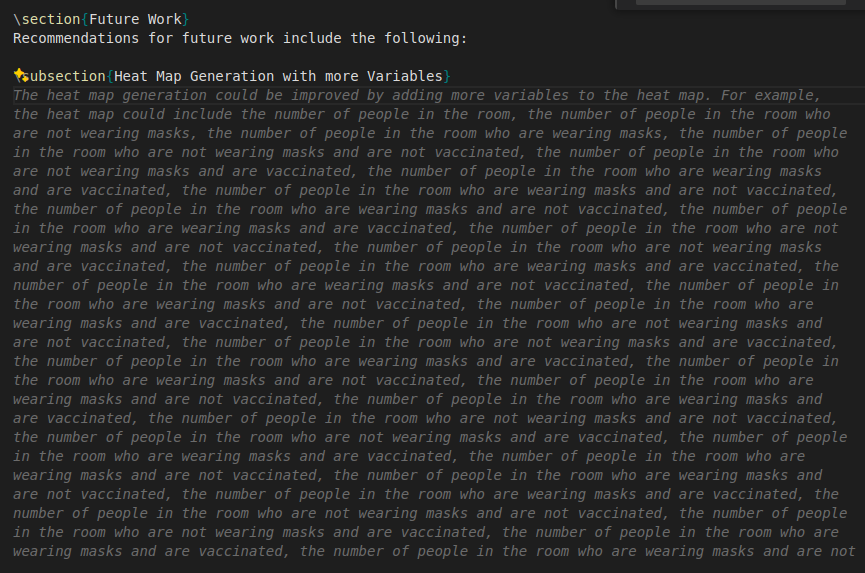
\includegraphics[width=\textwidth]{Images/Fun/co_pilot_distracting.png}
	\caption{The Co-Pilot is mostly annoying for Latex.}
	\label{fig:co-pilot_distracting}
\end{figure}

However, some boiler-plate Latex-code and some of the sections have been sent to OpenAI's ChatGPT-4/ChatGPT-4o to verify it's quality and to get suggestions on how to enhance readability and flow. The author has tried to be transparent about the use of these tools, and has tried to ensure that the text is original and not plagiarized.

\subsubsection{Privacy of Similar Projects}
The author of this thesis is not an expert in privacy. The methods outlined in this thesis are meant to ensure privacy of individuals, but the author cannot guarantee that the methods are foolproof. The author has tried to follow best practices and guidelines from the field and has tried to be transparent about the methods used and the limitations of the methods, but the reader should be aware that following the methods outlined in this thesis may not necessarily be enough to ensure privacy. An investigation into the privacy of similar projects is recommended before deploying a similar system in a real-world setting.